\begin{figure}[htb!]
  \begin{center}
    \resizebox{\textwidth}{!}{
      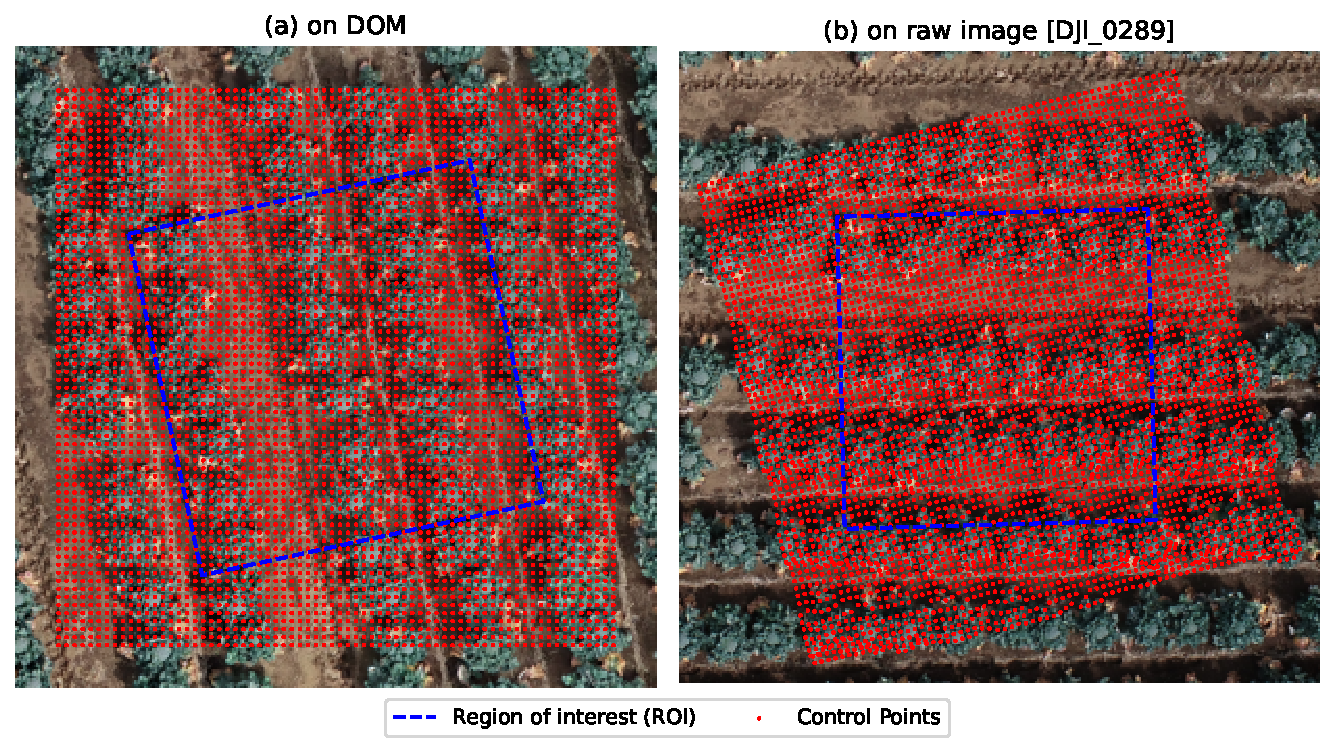
\includegraphics{figures/xrs/transform_cp_220331_114_DJI_0289.pdf}
    }
  \end{center}
  \caption[Control points between geographical coordinates on DOM and the pixel coordinate on raw image]{
    Control points between geographical coordinates on DOM and the pixel coordinate on raw image. The blue broken lines are the \gls{roi} boundary of the current grid, the red dots are the control points.
  }
  \label{fig:xrs2}
\end{figure}